% Section 7.1: acquisition strategies of the laboratory design study (main text: concepts only; settings in Appendix A).
% Facts: reports/2026-11_specimen/ldv_processing_log.md (items 30-31, 39-40, 50, 55, 59-62, 81, 89, 93, 96, 104-115)
% and reports/2026-11_mssp_paper/notes/run_list.md. Figure: src/ldv_pmma/plot_strategies.py -> F11_strategies.

\subsection{Acquisition strategies}\label{sec:lab-protocols}

Every strategy is replayed on the dense scan of Section~\ref{sec:experiment}: when a strategy asks for a position, it
receives the recording of the nearest scanned point, and nothing else. All strategies thus draw on the same data and
differ only in where they measure and how they turn their measurements into a map. A layout of 30 points costs about
\SI{2}{min} of scanning per shot, against about \SI{7}{h} for the dense scan.

The strategies differ in three choices (Fig.~\ref{fig:strategies}).
\begin{description}
\item[What is limited.] Either the \emph{scan budget}: 30 points in total, measured at once or in three batches of
  ten. Or the \emph{number of sensors}: 30 sensors that are moved and measured at five successive positions, which
  amounts to about 145 measured positions. The first mode corresponds to a scan whose cost is the number of points;
  the second to an array with a fixed number of channels that can be repositioned, as in the numerical study.
\item[Who decides where to measure.] No design (regular, jittered or random layouts, or random moves); a design made
  \emph{before} measuring, on the defect-free background model; or an \emph{adaptive} design, made between
  measurements on the model inverted from the data so far, with the illumination criterion of
  Section~\ref{sec:method}.
\item[How the map is made.] In \emph{one pass}, with all data at once and 100 updates, as for the dense scan; or
  \emph{staged}, with the updates interleaved with the measurements. Adaptive designs need the staged form, because
  each design step uses an intermediate model; the total number of updates is 100 in both cases.
\end{description}

\begin{figure}[ht]\centering
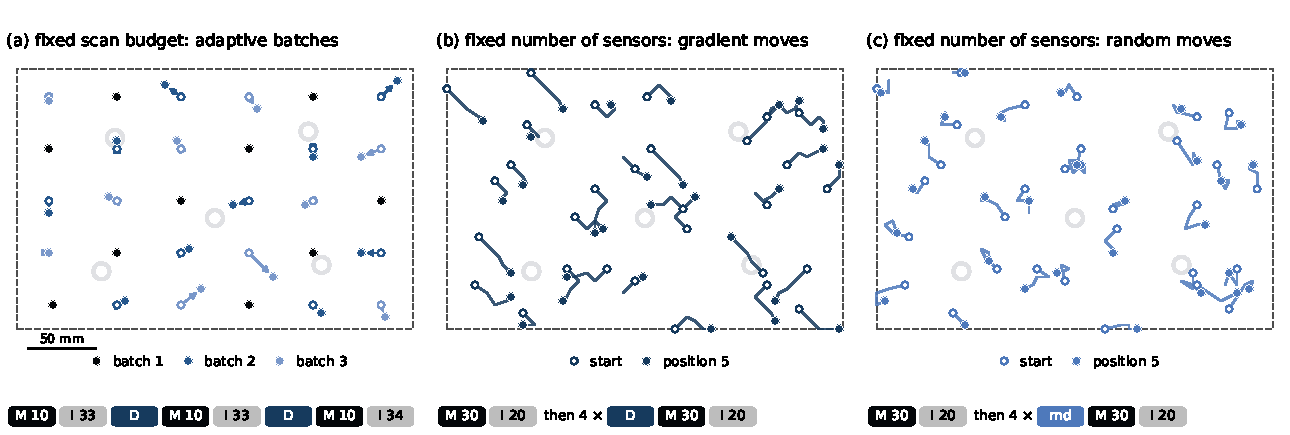
\includegraphics[width=\linewidth]{F11_strategies.pdf}
\caption{The two acquisition modes, drawn from three runs with four shots. (a) Fixed scan budget: 30 points in three
batches of ten; the first batch is measured as laid out, the next two are moved by the adaptive design (arrows, from the
planned to the measured position) on the model inverted from the batches before. (b) Fixed number of sensors: 30
sensors measured at five successive positions, each step following the illumination gradient on the current model.
(c) The same sensors and step lengths with random directions. Grey circles: the five features, for orientation only.
Bottom: sequence of measurements (M, number of points), inversion updates (I) and design steps (D) or random steps
(rnd).}\label{fig:strategies}
\end{figure}

Table~\ref{tab:strategies} places every strategy by the first two choices. Three further runs vary only the third:
\emph{progressive static} measures the static layouts in the same three batches with the staged inversion of the
adaptive batches; \emph{re-inversion} inverts the final 30 points of each adaptive run once, like a static layout; and
\emph{all visited positions} inverts the $\approx$145 positions of each moving array at once and compares them with a
static layout of the same size. All strategies are run with one, two and four shots from the same start layouts;
the settings are listed in Appendix~\ref{app:protocols}.

\begin{table}[ht]\centering\small
\caption{Strategies of the laboratory study, by what is limited and who places the points. Numbers: runs with four /
two / one shot.}\label{tab:strategies}
\begin{tabular}{@{}lll@{}}
\toprule
 & fixed scan budget (30 points) & fixed number of sensors (30 $\times$ 5 positions) \\ \midrule
no design            & static layouts \quad 8 / 7 / 7        & random moves \quad 3 / 5 / 5 \\
designed beforehand  & simulation design \quad 3 / 3 / 3 \note{24 Nov}  & offline moves \quad 3 / 5 / 5 \note{24 Nov} \\
adaptive             & adaptive batches \quad 5 / 5 / 4      & gradient moves \quad 3 / 5 / 5 \\
\bottomrule
\end{tabular}
\end{table}

The results are organised as three comparisons, from the most to the least permissive. In case (i), gradient moves
are compared with static layouts: the same number of sensors and the same inversion cost, but five times the scan.
In case (ii), adaptive batches re-inverted in one pass are compared with static layouts: the same scan cost, with
one extra inversion allowed. In case (iii), adaptive batches are compared with progressive static: the same scan and
the same inversion. Each step removes a possible source of advantage. In every case the controls with no design
(random moves, progressive static) and, where available, the designs made beforehand indicate how much of a
difference is due to adapting to the data.

Maps are scored with the two rules of Section~\ref{sec:scoring}: a fixed amplitude threshold, and detection at a
fixed false-indication rate. The comparison of gradient and random moves, and the tests of the adaptive batches
against static and progressive static layouts, were fixed before the runs they concern; the comparisons of cases (i)
and (ii) against static layouts and the fixed-rate rule were chosen after seeing results and are reported as
exploratory (Appendix~\ref{app:protocols}).
